\documentclass{standalone}
\usepackage{pgf}
\usepackage[english]{babel}
\usepackage[utf8]{inputenc}
%\usepackage{beamerthemesplit}
\usepackage{graphics,epsfig, subfigure}
\usepackage{url}
\usepackage{srcltx}
\usepackage{hyperref}
\usepackage{mathtools}
\usepackage{amsfonts}
\usepackage{amsmath}
\usepackage{physics}
\begin{document}
$
 \begin{aligned}
 	A_8^{\text{ans}}=\raisebox{-6.5mm}{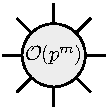
\includegraphics[trim={0cm 0cm 0cm 0cm},clip,scale=0.8]{8pt-contact}}\,+&\,\raisebox{-7.4mm}{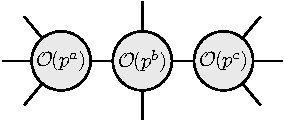
\includegraphics[trim={0cm 0cm 0cm 0cm},clip,scale=0.8]{8pt-double-fac}}\\
 	+\,\raisebox{-6.5mm}{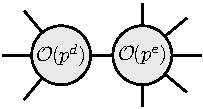
\includegraphics[trim={0cm 0cm 0cm 0cm},clip,scale=0.8]{8pt-single-fac}}&+\raisebox{-5.5mm}{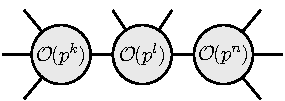
\includegraphics[trim={0cm 0cm 0cm 0cm},clip,scale=0.8]{8pt-double-fac-2}}.\label{Ans8pt}\\
 \end{aligned}
$
\end{document}